\section{Modelagem de escoamentos monofásicos}

%----------------------------------------------------------------------------------------

\begin{frame}{Modelagem de escoamentos monofásicos}
  Quando se aplica uma pressão (ou fluxo) em um domínio saturado por apenas \textbf{um fluido}, é induzido o que se chama de \textbf{escoamento monofásico}. A conservação de massa do fluido implica uma lei de balanço:

  \begin{equation}
      \frac{\partial}{\partial t}\int_V \phi\rho\ dx + \int_{\partial V}\rho (u \cdot n)\ ds = \int_V q\ dx.
  \end{equation}
  Aplicando-se o teorema da divergência, utilizando a Lei de Darcy e desenvolven-do-a, obtém-se a equação diferencial parcial de incógnitas $p$ e $\rho$:
  \begin{equation}
    \rho \phi c_t \frac{\partial p}{\partial t} - \nabla \cdot \left(\frac{\rho K}{\mu}(\nabla p - \rho g \nabla z)\right) = q,
  \end{equation}
  onde $c_t = c_f + c_r$ representa a compressibilidade total. Considerado um \textbf{escoamento incompressível}, a equação (\theequation)\ torna-se uma equação elíptica com coeficientes variáveis:
  \begin{equation}\label{eq246}
    - \nabla \cdot \left(\frac{\rho K}{\mu}(\nabla p - \rho g \nabla z)\right) = q.
  \end{equation}
\end{frame}

%----------------------------------------------------------------------------------------

\begin{frame}{Condições auxiliares}
  Além das equações que, de fato, modelam escoamentos monofásicos, faz-se necessário ainda condições de contorno. Estas condições podem ser classificadas principalmente em três tipos:

  \begin{itemize}
      \item \textbf{Dirichlet}, onde se dá pressão $p(x)$;
      \item \textbf{Neumann}, onde o fluxo $\nabla u \cdot n$ é dado; e
      \item \textbf{Robin} ou mista, onde é especificado $\alpha u + \beta (\nabla u \cdot n)$;
  \end{itemize}

  onde $u$ é uma função escalar, como por exemplo a temperatura ou pressão. Estas condições podem ser \textbf{homogêneas}, quando o contorno é igual a zero, ou \textbf{heterogêneas}, quando são iguais a uma função $g$.
\end{frame}

%----------------------------------------------------------------------------------------

\begin{frame}{Condições auxiliares}
  Para exemplificar os tipos de fronteiras nas bordas $\partial \Omega = \partial \Omega_p \cup \partial \Omega_u$, seguem as figuras:
    \begin{figure}[H]
    \centering
    \begin{subfigure}[b]{0.48\textwidth}
      \centering
      \begin{tikzpicture}[scale=1.6]
        \fill[fill=orange!40] (-1,-1) rectangle (1,1);
        \node[font=\Large] at (0,0) {$\Omega$};
        
        \node[left, above, font=\small] at (-1,1) {$\partial \Omega$};
        \fill[pattern=north east lines, pattern color=gray!80] (1,-1.1) rectangle (1.1,1.1);
        \draw[thick] (1,-1.1) -- (1,1.1);
        \draw[black] (-1,-1) rectangle (1,1);

        \node[rotate = 90, right, anchor=center] at (1.3,0) {$p(x,y) = 0$};
      \end{tikzpicture}
      \caption{Contorno Dirichlet homogêneo.}
    \end{subfigure}
    \hfill
    \begin{subfigure}[b]{0.48\textwidth}
      \centering
      \begin{tikzpicture}[scale=1.6]
        \fill[fill=orange!40] (-1,-1) rectangle (1,1);
        \node[font=\Large] at (0,0) {$\Omega$};
        
        \node[left, font=\small] at (-1,1) {$\partial \Omega$};
        \fill[pattern=north east lines, pattern color=gray!80] (-1.1,-1) rectangle (1.1,-1.1);
        \draw[thick] (-1.1,-1) -- (1.1,-1);
        \draw[black] (-1,-1) rectangle (1,1);

        \foreach \y in {-0.8,-0.4,0.0,0.4,0.8}
        {
          \draw[->, thick, black!60] (\y,-.9) -- (\y,-1.1);
        }

        \node[below, anchor=center] at (0,-1.5) {$-K\frac{\partial p}{\partial n} = g(x,y)$};
      \end{tikzpicture}
      \caption{Contorno Neumann não homogêneo.}
    \end{subfigure}
    \caption{Exemplificação de tipos de contorno.}
  \end{figure}
\end{frame}

%----------------------------------------------------------------------------------------

\begin{frame}{Meios homogêneos e heterogêneos}
  Para classificar meios como homogêneos ou heterogêneos, considera-se uma simplificação de \eqref{eq246}\ para o escoamento monofásico, com as hipóteses do escoamento ser \textit{incompressível, isotérmico e sem efeito gravitacional}, da forma que:
  \begin{equation}\label{escoamento_base}
  \left\{
    \begin{aligned}
      \nabla \cdot u &= \frac{q}{\rho} && \text{em } \Omega \\
      u &= -\frac{K}{\mu} \nabla p && \text{em } \Omega \\
      p &= p_b && \text{em } \partial\Omega_p \\
      u \cdot n &= u_b && \text{em } \partial\Omega_u
    \end{aligned}
  \right.
  ,
  \end{equation}
  onde a viscosidade $\mu$ e massa específica $\rho$ são uniformes no caso incompressível e consideradas unitárias aqui. Também, onde $\partial \Omega = \partial \Omega_p \cup \partial \Omega_u$ é a fronteira do domínio $\Omega \subset \mathbb{R}^d$ com $d = \{1,2,3\}$.
\end{frame}

%----------------------------------------------------------------------------------------

\begin{frame}{Meios homogêneos e heterogêneos}
  Portanto, o meio pode ser classificado, principalmente entre:
  \begin{itemize}
    \justifying
    \item Um meio dito \textbf{homogêneo}, governado pelo sistema de escoamentos mono-fásicos (\theequation), ocorre quando a permeabilidade absoluta $K$ é constante e uniforme, logo não dependendo de $x$; ou
    \item Quando o meio é \textbf{heterogêneo}, a permeabilidade absoluta $K$ varia com $x$ e então o escoamento tende a passar pelas regiões de alta permeabilidade e evitar as de baixa permeabilidade.
  \end{itemize}
  Também, é possível usar um modelo do projeto \textit{SPE10} fornecido pela \textit{Sociedade de Engenheiros de Petróleo}, utilizado como referência em simulações de reservatórios de petróleo.
\end{frame}

%----------------------------------------------------------------------------------------

\begin{frame}{Método de volumes finitos}
  O \textbf{método de volumes finitos} é um método de discretização útil para simulações numéricas de leis de conservação de vários tipos: \textit{elípticas, hiperbólicas ou parabólicas}, por exemplo. Este método tem alguns pontos importantes: 
  \begin{itemize}
    \justifying
    \item Pode ser usado em \textbf{geometrias arbitrárias};
    \item Pode ser usado em \textbf{malhas estruturadas ou não}; e
    \item \textbf{Conserva localmente os fluxos numéricos}, o que o faz particularmente interessante para problemas de mecânica dos fluidos.
  \end{itemize}
  Isso pode ser obtido, pois é baseado em uma abordagem "balanceada":
  \begin{itemize}
    \justifying
    \item Um {balanço local} é escrito em cada célula de discretização, que é frequentemente chamada de \textit{volume de controle};
    \item Pela fórmula de divergência, uma {formulação da integral} dos fluxos sobre a fronteira do volume de controle é obtida.
  \end{itemize}
  Os fluxos nas fronteiras são discretizados com respeito aos discretos "desconhecidos".
\end{frame}

%----------------------------------------------------------------------------------------

\begin{frame}{Malha centrada em células}
  Durante o restante desse trabalho, será usada uma discretização \textbf{centrada em células}, onde é considerado que o \textit{valor aproximado da função}, ou da média dos valores da célula, \textit{está justamente no centro dela}.

  Para visualizar melhor, toma-se o intervalo $I = [0,1]$ com três subintervalos de espaçamento uniforme:
  \begin{figure}[H]
    \centering
    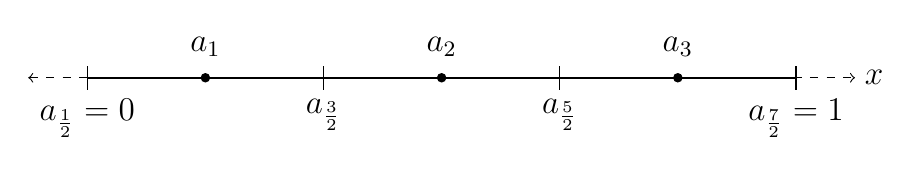
\begin{tikzpicture}[scale=1.5]
      % Eixo x
      \draw[black, dashed, <->] (-.5,0) -- (6.5,0);
      \draw[black,thick] (0,0) -- (6,0);
      
      % Linhas da malha
      \filldraw[black] (1,0) circle (1pt);
      \filldraw[black] (3,0) circle (1pt);
      \filldraw[black] (5,0) circle (1pt);

      \node[above, font=\large] at (1,0.1) {$a_{1}$};
      \node[above, font=\large] at (3,0.1) {$a_{2}$};
      \node[above, font=\large] at (5,0.1) {$a_{3}$};

      \draw[black]     (0,-0.1) -- (0,0.1);
      \draw[black]     (2,-0.1) -- (2,0.1);
      \draw[black]     (4,-0.1) -- (4,0.1);
      \draw[black]     (6,-0.1) -- (6,0.1);

      \node[below, font=\large] at (0,-0.1) {$a_{\frac{1}{2}} = 0$};
      \node[below, font=\large] at (2,-0.1) {$a_{\frac{3}{2}}$};
      \node[below, font=\large] at (4,-0.1) {$a_{\frac{5}{2}}$};
      \node[below, font=\large] at (6,-0.1) {$a_{\frac{7}{2}} = 1$};

      \node[right, font=\large] at (6.5,0) {$x$};

    \end{tikzpicture}
    \caption{Intervalo $I$ com discretização no centro da célula e contorno de Neumann.}
    \label{fig:viz_CCG_N}
  \end{figure}
  Os valores dos nós $a_i$ são vistos como os \textbf{centros} das células, então $a_{i-1/2}$ e $a_{i+1/2}$ seriam suas faces à esquerda e à direita. No caso de \textit{contornos de Neumann} na primeira célula, durante a integração de $[a_{\frac{1}{2}},a_{\frac{3}{2}}]$, o fluxo vindo de $a_{\frac{1}{2}}$ seria a \textit{imposição de fluxo da interface esquerda} do contorno de Neumann. 
\end{frame}

%----------------------------------------------------------------------------------------

\begin{frame}{Malha centrada em células}
  Geralmente, nos contornos de Dirichlet, inclui-se uma \textbf{célula fantasma} como na figura abaixo:
  \begin{figure}[H]
    \centering
    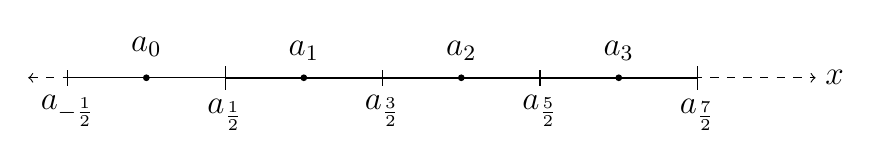
\begin{tikzpicture}[scale=1]
      % Eixo x
      \draw[black, dashed, <->] (-2.5,0) -- (7.5,0);
      \draw[black]              (-2,  0) -- (0,  0);
      \draw[black,thick]        ( 0,  0) -- (6,  0);
      % Linhas da malha
      \filldraw[black] (-1,0) circle (1pt);
      
      \filldraw[black] (1,0) circle (1pt);
      \filldraw[black] (3,0) circle (1pt);
      \filldraw[black] (5,0) circle (1pt);

      \node[above, font=\large] at (-1,0.15) {$a_{0}$};

      \node[above, font=\large] at (1,0.1) {$a_{1}$};
      \node[above, font=\large] at (3,0.1) {$a_{2}$};
      \node[above, font=\large] at (5,0.1) {$a_{3}$};

      \draw[black] (-2,-0.1) -- (-2,0.1);

      \draw[black] ( 0,-0.15) -- ( 0,0.15);
      \draw[black] ( 2,-0.1) -- ( 2,0.1);
      \draw[black] ( 4,-0.1) -- ( 4,0.1);
      \draw[black] ( 6,-0.15) -- ( 6,0.15);

      \node[below, font=\large] at (-2,-0.1) {$a_{-\frac{1}{2}}$};

      \node[below, font=\large] at (0,-0.15)  {$a_{\frac{1}{2}}$};
      \node[below, font=\large] at (2,-0.1)  {$a_{\frac{3}{2}}$};
      \node[below, font=\large] at (4,-0.1)  {$a_{\frac{5}{2}}$};
      \node[below, font=\large] at (6,-0.15)  {$a_{\frac{7}{2}}$};

      \node[right, font=\large] at (7.5,0) {$x$};

    \end{tikzpicture}
    \caption{Intervalo $I$ com discretização no centro da célula, contorno de Dirichlet à esquerda usando célula fantasma.}
    \label{fig:viz_CCG_D}
  \end{figure}

  No exemplo do intervalo $I$ descrito, a célula fantasma seria a célula com centro em $a_0$, então se utilizando desse valor na integração em $[a_{\frac{1}{2}},a_{\frac{3}{2}}]$. Por simplicidade, o contorno à direita se manteve de Neumann.

  Também, é possível usar meia célula, como em:
  \begin{figure}[H]
    \centering
    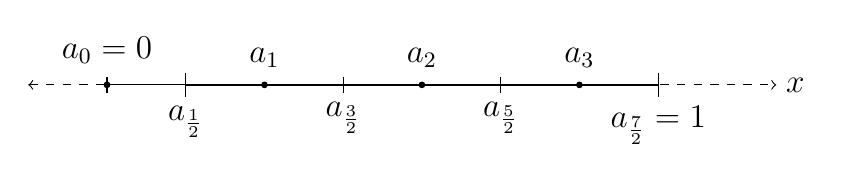
\begin{tikzpicture}[scale=1]
      % Eixo x
      \draw[black, dashed, <->] (-2.0,0) -- (7.5,0);
      \draw[black]              (-1,  0) -- (0,  0);
      \draw[black,thick]        ( 0,  0) -- (6,  0);
      % Linhas da malha
      \filldraw[black] (-1,0) circle (1pt);
      
      \filldraw[black] (1,0) circle (1pt);
      \filldraw[black] (3,0) circle (1pt);
      \filldraw[black] (5,0) circle (1pt);

      \node[above, font=\large] at (-1,0.15) {$a_{0} = 0$};

      \node[above, font=\large] at (1,0.1) {$a_{1}$};
      \node[above, font=\large] at (3,0.1) {$a_{2}$};
      \node[above, font=\large] at (5,0.1) {$a_{3}$};

      \draw[black] (-1,-0.1) -- (-1,0.1);

      \draw[black] ( 0,-0.15) -- ( 0,0.15);
      \draw[black] ( 2,-0.1) -- ( 2,0.1);
      \draw[black] ( 4,-0.1) -- ( 4,0.1);
      \draw[black] ( 6,-0.15) -- ( 6,0.15);

      \node[below, font=\large] at (0,-0.15) {$a_{\frac{1}{2}}$};
      \node[below, font=\large] at (2,-0.1 ) {$a_{\frac{3}{2}}$};
      \node[below, font=\large] at (4,-0.1 ) {$a_{\frac{5}{2}}$};
      \node[below, font=\large] at (6,-0.15) {$a_{\frac{7}{2}} = 1$};

      \node[right, font=\large] at (7.5,0) {$x$};

    \end{tikzpicture}
    \caption{Intervalo $I$ com discretização no centro da célula, contorno de Dirichlet à esquerda usando meia célula.}
    \label{fig:viz_CCG_Dh}
  \end{figure}
\end{frame}

%----------------------------------------------------------------------------------------